\documentclass{jdrp}

\bibliography{songes-de-l-uhumele/references} 

\newcommand*{\crg}{{\aurebesh\Large \$}} % Symbol for Galactic Credits

\hypersetup{
	pdftitle={SWR - Songes de l’Uhumele},
	pdfsubject={Scénario, Songes de l’Uhumele},
	pdfauthor={Marthym},
	pdfkeywords={starwars,savage,worlds,jdr,scenario},
	pdfcopyright={This work is licensed under the Creative Commons Attribution-ShareAlike 4.0 International License.}
}

\begin{document}

	\begin{titlepage}

	\begin{center}
		\hspace*{\vfill}
		\noindent\Huge\jedifont{Star Wars Redemption}\\ 
		\noindent\fontsize{50}{70}\jedifont{\$}
		\noindent\fontsize{50}{70}\jedifont{\#}\\
		\noindent\fontsize{40}{60}\jedifont{Songes de l’uhumele}
		\hspace*{\vfill}
	\end{center}

	%\hspace*{\vfill}

	\noindent\makebox[\textwidth]{
		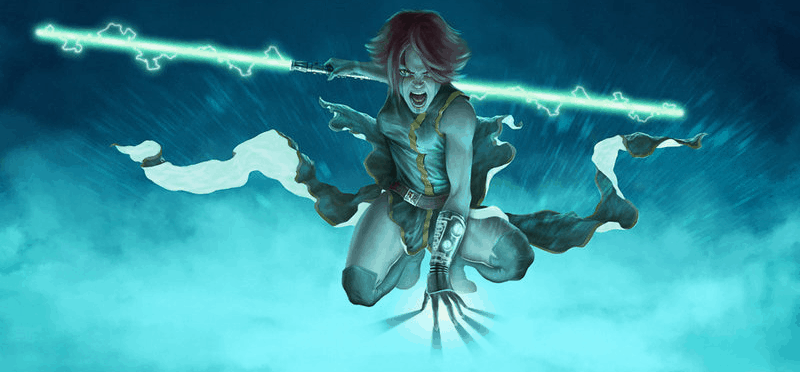
\includegraphics[width=\paperwidth]{_img/cover-bg.png}}
	\begin{tikzpicture}[overlay]
		\node[minimum width=180pt,minimum height=180pt, rotate=30] at (15,11){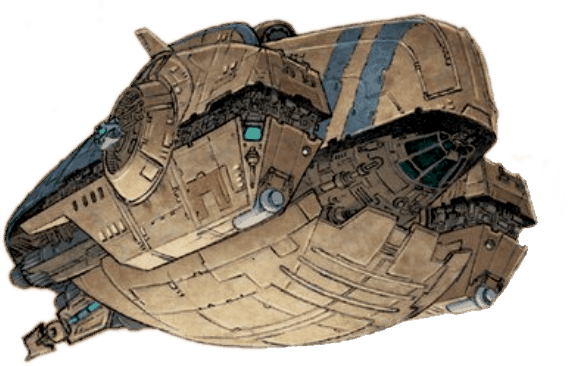
\includegraphics[width=180pt]{_img/songes-de-l-uhumele/uhumele.png}};
	\end{tikzpicture}}
	\end{titlepage}

	\onecolumn
	\section{Contexte du Scénario}
	
	Voici un court scénario sur le thème de \nameref{sec:uhumele}. Ce scénario bien qu’indépendant est fortement lié à la campagne "Dos au Muur" de \citetitle{jdrp-starwars}. C’est un scénario écrit pour pour faire patienter entre deux étapes de la campagne (2 et 3). 

	L’idée est que l’un des personages, sensible à la force et possédant \textit{Sens de Force} a une vision d’un évènement passé. En l’occurence, la tentative de sauvetage de Resa, la fille de \textbf{Bomo Greenbark} par l'équipage de l’Uhumele. Les joueurs jouent alors le rôle des membres de l’équipage (avec leur propre fiche de perso). Ce système à l’intéret d’introduire l’Uhumele dans la campagne Dos au Muur mais aussi de ne pas modifier les circonstances entre les 2 scénarios. Pas besoin de faire des raccords tiré par les cheveux.

	Biensûr, ce scénario peut aussi être joué hors du contexte de la campagne Dos au Muur, en remplaçant l’introduction "vision" par, par exemple, une introduction à base de contrat.

	A noter que ce scénario est plutôt fait pour des héros notre ou orienté gentils. 

	Ce scénario se passe normalement en -19 pendant les derniers affrontements entre l’armée des clones et les armées de droïde de la Confédération des Systèmes Indépendants.

	\twocolumn

	\section{introduction}
	L’équipage de \nameref{sec:uhumele} quitte Nouvelle Plympto au lendemain d’une grande bataille qui a obligé les habitants a évacuer pour se mettre à l’abri. \'A cette époque, l’équipage du Uhumele venait de mettre la main sur une cargaison inconnue et dangeureuse qui les pousse à éviter l’Empire au maximum. C’est pourquoi quand l’Empire est arrivé pour s’opposer aux droïdes, le vaisseau a quitté la planête en urgence. Mais dans la précipitation, la famille de \textbf{Bomo Greenbark} n’a pas eu le temps d’embarquer dans l’Uhumele et s'est trouvée évacuée par l’Empire. 

	Quand Bomo se renseigne pour savoir sur quel vaisseau a été évacué sa famille, il apprend que sa femme et sa fille ont embarqué sur le \textbf{Sevarog} un vaisseau à destination d’Orvax IV, plate-forme galactique majeure du trafic d’esclaves. Le scénario commence au moment où Bomo demande de l’aide à l’équipage de l’Uhumele pour récupérer sa fille.

	\section{orvax iv}
	Plate-forme galactique majeure du trafic d’esclaves, Orvax IV est situé dans la bordure extérieur et peuplé d’à peu près toutes les espèces que compte la galaxie. L’Empire comme la République ne s’y sont jamais intéressé et laisse cette planète faire ses affaire comme elle le souhaite.

	La planète se présente comme un vaste marché aux esclaves, trié en catégorie, races, age, genre, \ldots.

	Première étape, retrouver le \textbf{Sevarog} à bord duquel est arrivée la famille de Bomo. N’importe qui au spacioport donnera le numéro du quai où se trouve le vaisseau. Bien sur, les esclaves ont été débarqués et la famille de Bomo ne se trouve plus à bord. S’il l'interroge, le capitaine du Sevarog apprend que les esclaves déportés par l’Empire sont stocké dans un fosse au nord du spacioport en dessous de la boutique "U2".

	\section{Fosse u2}
	En tant qu’entrepot de stockage de l’Empire, la zone est sous bonne garde, des \nameref{sec:storm-trooper}s patrouilles régulièrement dans le coin et l’arrière de la boutique est gardé.

	\section{Annexes}
	\subsection{l’Uhumele}\label{sec:uhumele}


	\section{Bestiaire}

\subsection{Rakghoul}
\label{sec:rakghoul}
\noindent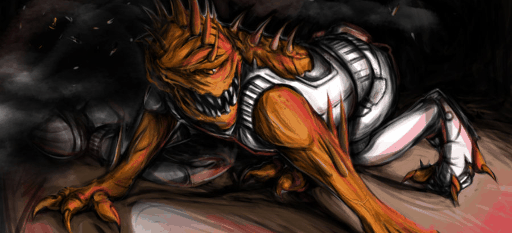
\includegraphics[width=\linewidth]{_img/dos-au-muur/rakghoul.png}

\subsubsection{Traits}

\begin{itemtable}[ c c c c c ]
    \textbf{Agi} & \textbf{Int} & \textbf{\^Ame} & \textbf{For} & \textbf{Vig} \\
    d8           & d6           & d6             & d8           & d8
\end{itemtable}
\begin{itemtable}[ l X ]
    \textbf{Allure}      & 6 \\
    ~                    & Vision Nocturne \\
    ~                    & Marche sur les murs \\
    \textbf{Compétences} & Combat d8, Discrétion d6
\end{itemtable}

\subsubsection{Défense}
\begin{itemtable}[ c c ]
    \textbf{Parade}     & \textbf{Résistance} \\
    6                   & 6 
\end{itemtable}

\subsubsection{Attaque}
\begin{itemtable}[ X c c ]
    ~       & \textbf{Combat}   & \textbf{Dégats} \\
    Griffes & d8                & 1d6 
\end{itemtable}

\newpage
\subsubsection{Background}
Les Rakghouls sont une espèce issue d’une maladie créée par le seigneur Sith Karness Muur. Les individus atteint par cette maladie deviennent des monstres incapables de penser par eux-mêmes. Karness peut les contrôler grâce à son talisman (Le Talisman de Muur).

La maladie se transmet par une griffure ou une morsure mais cela ne fonctionne pas avec les êtres sensibles à la Force. Karness a créé ce virus à partir du coté Obscur de la Force ce qui explique une forte présence obscure près de ces monstres.

Karness a créé plusieurs versions du virus car les premiers Rakghouls ne répondaient pas bien au contrôle de Karness. Les nouveaux sont plus réceptifs et plus fort.

Quand le Talisman de Muur a été perdu dans les bas fonds de Taris, on a peu constaté que les créatures, suite à une exposition prologée au Talisman finissaient par se transformer en Rakghouls. Mais les Rakghouls transformé de cette façon sont bestiaux, stupides et sans âme. Ils attaquent tout ce qui bouge. Ces créatures ne fonctionnent qu’à l’instinct.

\clearpage
\subsection{Rakghoul Amblyope}
\label{sec:rakghoul-amblyope}
\noindent
\includegraphics[width=\linewidth]{_img/dos-au-muur/rakghoul-amblyope.png}

\subsubsection{Traits}

\begin{itemtable}[ c c c c c ]
    \textbf{Agi} & \textbf{Int} & \textbf{\^Ame} & \textbf{For} & \textbf{Vig} \\
    d4           & d6           & d6             & d12+2        & d10
\end{itemtable}
\begin{itemtable}[ l X ]
    \textbf{Allure}      & 5 \\
    \textbf{Taille}      & +5 \\
    ~                    & Vision de Force \\
    ~                    & \'Enorme (+2 pour les jets d’attaque adverses)\\
    \textbf{Compétences} & Combat d10
\end{itemtable}

\subsubsection{Défense}
\begin{itemtable}[ c c ]
    \textbf{Parade}     & \textbf{Résistance} \\
    5                   & 12 
\end{itemtable}

\subsubsection{Attaque}
\begin{itemtable}[ X c c ]
    ~           & \textbf{Combat}   & \textbf{Dégats} \\
    Mains nues  & d10               & d12+2 
\end{itemtable}

\newpage
\subsubsection{Background}
Version stéroïdée des Rakghouls standard, Amblyope est notre petit boss de niveau.

Quand les Rakghouls sont livrés à eux-mêmes et qu’ils laissent libre cours à leurs plus bas instincts, il arrive qu’un Rakghoul plus fort que les autres s’en prenne à ces petits camarades et les dévore sans scrupules. Cet afflux de Force Obscure peut le faire muter et le Rakghoul devient une espèce de gros monstre de 3m de haut, complètement aveugle mais attiré par les émanations de Force, il attaque machinalement les adversaires les plus sensibles à la Force. 

\clearpage

\subsection{Contrebandier (Taris)} \label{sec:taris-contrebandier}
\noindent
\includegraphics[width=\linewidth]{_img/dos-au-muur/contrebandier.png}

\subsubsection{Traits}

\begin{itemtable}[ c c c c c ]
    \textbf{Agi} & \textbf{Int} & \textbf{\^Ame} & \textbf{For} & \textbf{Vig} \\
    d6           & d6           & d4             & d8           & d8
\end{itemtable}
\begin{itemtable}[ l X ]
    \textbf{Allure}      & 6 \\
    \textbf{Compétences} & Combat d8, Tir d10
\end{itemtable}

\subsubsection{Défense}
\begin{itemtable}[ c c ]
    \textbf{Parade}     & \textbf{Résistance} \\
    5                   & 6 (+1)
\end{itemtable}

\subsubsection{Attaque}
\begin{itemtable}[ X c c ]
    ~           & \textbf{Combat}   & \textbf{Dégats} \\
    Blaster     & -                 & 2d6+1
\end{itemtable}

\newpage
\subsubsection{Background}
Les bas-fonds de Taris grouillent de toutes sortes de malfrats. C’est un des coins favoris de contrebandiers qui peuvent y kidnapper de jeunes enfants en toute impunité. Personne ne viendra se plaindre de la disparition d’une vermine de plus dans les bas fond.

Ce ne sont en général que des débutants attiré par la facilité. Seul ils ne représentent pas un grand danger, mais ils se promènent souvent en groupe.

\clearpage

\subsection{Storm Trooper} \label{sec:storm-trooper}
\noindent
\includegraphics[width=\linewidth]{_img/dos-au-muur/stormtrooper.png}
\newpage
\subsubsection{Traits}

\begin{itemtable}[ c c c c c ]
    \textbf{Agi} & \textbf{Int} & \textbf{\^Ame} & \textbf{For} & \textbf{Vig} \\
    d4           & d6           & d4             & d8           & d8
\end{itemtable}
\begin{itemtable}[ l X ]
    \textbf{Allure}      & 6 \\
    \textbf{Compétences} & Combat d10, Tir d10
\end{itemtable}

\subsubsection{Défense}
\begin{itemtable}[ c c ]
    \textbf{Parade}     & \textbf{Résistance} \\
    7                   & 6 (+4)
\end{itemtable}

\subsubsection{Attaque}
\begin{itemtable}[ X c c ]
    ~              & \textbf{Combat}   & \textbf{Dégats} \\
    Fusil Blaster  & -                 & 2d8 (3)
\end{itemtable}

\subsubsection{Background}
Soldats dévoué de l’empire. Certain sont des clones restant de la guerre des clones d’autres non. Ils sont entrainés au combat, équipé d’une bonne armure et armé de Fusil Blaster efficaces.

\clearpage
\subsection{Wampa} \label{sec:wampa}

\clearpage
\subsection{Cybercleps} \label{sec:cybercleps}

	\onecolumn
	\nocite{*}
	\printbibliography
\end{document}